\chapter{The Transcorrelated Method for Multireference Problems}
\label{chap:binding}

This chapter is based in large part on the following upcoming publication:\\
\fullcite{haupt_sizeconsistent}

Images have been reused from this paper (with permission).

\section{Introduction}

In this chapter, we apply the new framework for the transcorrated method described in chapter \ref{chap:opt} to problems of multireference character and find these methods may yield non-physical results. We propose an updated workflow wherein we use conventional post-Hartree-Fock methods as input to Jastrow optimisation for TC-FCIQMC. Results suggest size-consistent results and rapid basis set convergence compared to conventional methods, with the binding curve of N$_2$ at \avtz being within chemical accuracy of experiment.

\section{Motivation}

A popular ``stress test'' for quantum chemistry methods is the binding curve of N$_2$. Highly accurate experimental results\supercite{leroyAccurate2006} exist to recreate the curve, allowing for a useful benchmark. At equilibrium, this system is essentially single reference in character, but as the bond is stretched, the system becomes strongly multireference, making it particularly challenging for many methods. As an example, we might consider standard \gls{CCSD}, which is a single-reference method, compared to FCIQMC which (within stochastic error) is exact. Figure \ref{fig:ccsd-vs-fciqmc-n2} shows the binding curve of N$_2$ with CCSD compared to FCIQMC, using \avtz. We see that CCSD is not stable at large bond lengths.

\begin{figure}[htbp]
    \centering
    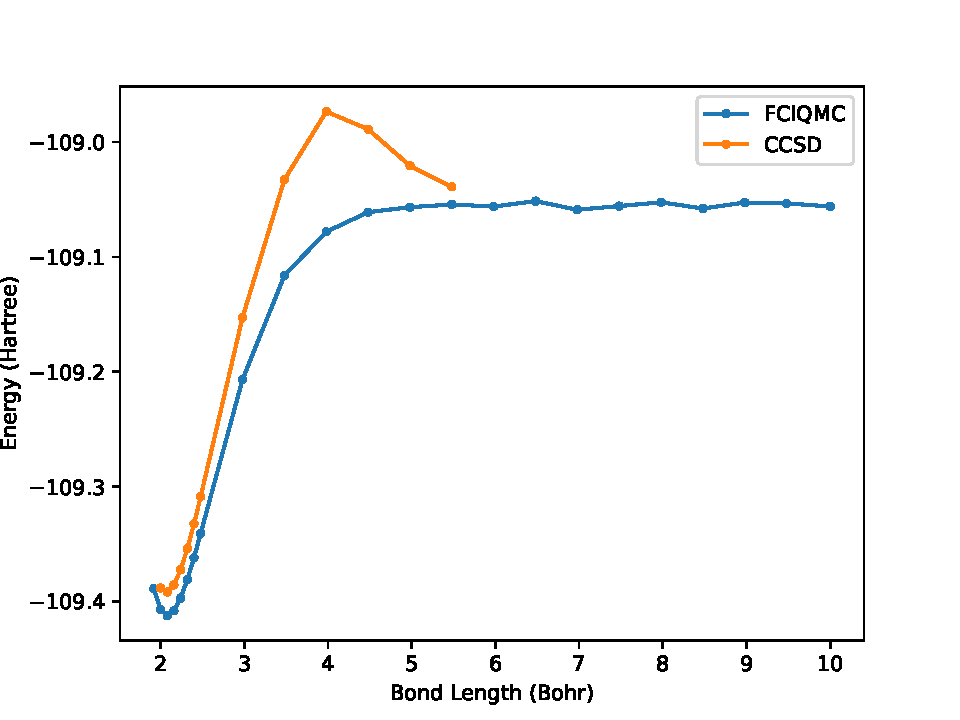
\includegraphics[width=0.8\textwidth]{figures/binding/N2_avtz_nontc}
    \caption{The binding curve for N$_2$ with the \avdz basis set. CCSD starts to decrease near 4 Bohr, which is nonphysical, whereas FCIQMC provides a more accurate curve. FCIQMC was done with 30 million walkers and HF-projected energy. The nonsmooth points in the dissociated region is due to stochastic error, and could be resolved with more walkers and a better trial wave function. CCSD did not converge at bond lengths larger than those shown.}
    \label{fig:ccsd-vs-fciqmc-n2}
\end{figure}

To see how well TC fares against such problems, consider the methodology outlined in chapter \ref{chap:opt}. We again use the same Jastrow factor as in equation \ref{eq:jastrow},
\begin{equation}
    \label{eq:jastrow-again}
    J = \sum_{i<j}^Nv(r_{ij}) + \sum_i^N\sum_I^{N_A}\chi(r_{iI}) + \sum_{i<j}^N\sum_I^{N_A}f(r_{ij}, r_{iI}, r_{jI}),
\end{equation}
with
\begin{equation}
    \label{eq:dtn-jastrow-ee-2}
    v(r_{ij})    = t(r_{ij},L_v)
                    \sum_{k} a_k r_{ij}^k ,
\end{equation}
\begin{equation}
    \label{eq:dtn-jastrow-en-2}
    \chi(r_{iI}) = t(r_{iI},L_\chi)
    \sum_{k} b_k r_{iI}^k ,
\end{equation}
\begin{equation}
    \label{eq:dtn-jastrow-een-2}
    f(r_{ij}, r_{i}, r_{j}) = t(r_{iI},L_f) t(r_{jI},L_f)
    \sum_{k,l,m} c_{klm}
    r_{ij}^k r_{iI}^l r_{jI}^m ,
\end{equation}
and the same cutoff functions $t(r,L) = (1-r/L)^3
\Theta(r-L)$. We also use the same objective function,
\begin{equation}
    \label{eq:varref-hf}
    \sigma_\mathrm{ref}^2 = \sum_{I\neq \mathrm{HF}}\bra{D_I}\htc\ket{D_\mathrm{HF}},
\end{equation}
Using this workflow with the xTC approximation, we calculate points along the binding curve of N$_2$, and find a non-physical ``dip'', as shown in figure \ref{fig:binding-dip}, similar to what CCSD exhibits in figure \ref{fig:ccsd-vs-fciqmc-n2}, albeit much more subtle.

\begin{figure}[htbp]
    \centering
    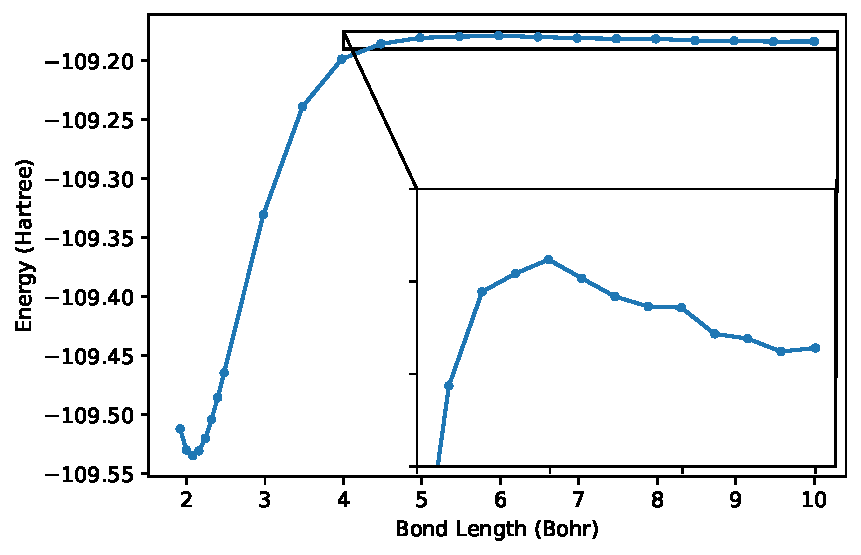
\includegraphics[width=0.8\textwidth]{figures/binding/inset_nontcfciqmc}
    \caption{The xTC-FCIQMC binding curve for N$_2$ with the \avtz basis set. While much smaller than that in figure \ref{fig:ccsd-vs-fciqmc-n2}, a non-physical dip is still present. This is apparent when zooming in on the curve, as shown in the inset.}
    \label{fig:binding-dip}
\end{figure}

This result has been verified for a few points with full TC (that is, with no approximations), which rules out xTC as the issue. Since the post-Hartree-Fock treatment was essentially at the FCI level, this implies that there is something wrong with the calculation of the Jastrow factors themselves. That is, our Hamiltonian is already ``corrupted'' before we even start the post-HF calculation.


\section{Resolving the Problem}

Based on the discussion in the previous section, it is likely that the transcorrelated workflow suffers from a single-reference bias. Indeed, the clear culprit is the Slater-Jastrow ansatz
\begin{equation}
    \label{eq:slater-jastrow}
    \Psi_\mathrm{SJ} = \e^J\Phi_\mathrm{HF},
\end{equation}
which affects the Jastrow optimisation and in turn the TC Hamiltonian $\htc = e^{-J}\hat H\e^J$.

We modify equation \ref{eq:slater-jastrow} to optimise for a multireference expansion,
\begin{equation}
    \label{eq:general-slater-jastrow}
    \Psi = \e^J\Phi_0
\end{equation}
where $\ket{\Phi_0}=\sum_I\ket{D_I}$. In practice, this modification results in two key changes in the workflow:
\begin{itemize}
    \item The objective function used during the VMC optimisation, equation \ref{eq:varref-hf}, needs to reflect the multireference ansatz. In particular, it will need to be changed to
    \begin{equation}
        \label{eq:varref-md}
        \sigma_\mathrm{ref}^2 = \sum_{I}\bra{D_I}\htc\ket{\Phi_0} - \bra{\Phi_0}\htc\ket{\Phi_0},
    \end{equation}
    which is evaluated in VMC by sampling
    \begin{equation}
        S_\mathrm{ref}^2 =
          \frac 1 {n_\mathrm{opt}-1}
          \sum_{n=1}^{n_\mathrm{opt}}
            \left| \frac {\hat H({\bm R}_n) \Psi({\bm R}_n)}
                         {\Psi({\bm R}_n)} - {\bar E}_\mathrm{ref}
            \right|^2.
    \end{equation}
    \item The density matrices used for xTC during integration must reflect this change as well. In particular, $\gamma_{p\dots}^{q\dots}=\bra{\Phi_0} a_{p\dots}^{q\dots}\ket{\Phi_0}$ in the equations in section \ref{sec:xtc}.
\end{itemize}

\subsection{Size Consistency}

One possible concern when studying problems like dissociation is that the method be size consistent. It is worth noting that one of the earliest Jastrow factors used for TC\supercite{boysCalculation1969} as well as in more recent work\supercite{cohenSimilarity2019} is given by
\begin{equation}
\label{eq:boyshandyjastrow}
J = \sum_{i<j} u(\bm r_i, \bm r_j)
\end{equation}
where
\begin{equation}
u(\bm r_i, \bm r_j) = \sum_{l,m,n}^{m+n+o\leq 6} c_{lmn}(\bar r_{iM}^m\bar r_{jN}^n+\bar r_{jM}^m\bar r_{iN}^n)\bar r_{ij}^l
\end{equation}
and $\bar r = r/(1+r)$.
However, notice that for $l=0$ and $n,m>0$, we can have non-vanishing gradients of $u$ for arbitrary distances between $N$ and $M$, and hence for systems $A$ and $B$ arbitrarily far apart we do not necessarily have
\begin{equation}
\label{eq:size-consistency}
e^{J_{A+B}}\ket{\Phi_{A+B}} = e^{J_0}(e^{J_{A}}\ket{\Phi_{A}})(e^{J_{B}}\ket{\Phi_{B}}),
\end{equation}
as $J_A$ will still act on system $B$, and vice versa. Here, $J_0$ is the electron-electron part of the Jastrow factor, $J_A$ the part involving nuclei in system $A$, and $J_B$ terms involving nuclei in system $B$.

In contrast to these previous works, our Jastrow ansatz, equation \ref{eq:jastrow-again}, first presented by Drummond, Towler and Needs,\supercite{drummondJastrow2004} vanishes when systems $A$ and $B$ are far apart due to the presence of the cutoff functions. Therefore, our Jastrow factor form does not suffer from this problem.

We must also ensure size consistency in our optimisation procedure. Assuming $\Phi_0$ is itself size consistent, it follows that for the given $J$, for non-interacting systems $A$ and $B$, the objective function, equation \ref{eq:varref-md}, $\sigma_\mathrm{ref}^2(A+B) = \sigma_\mathrm{ref}^2(A) + \sigma_\mathrm{ref}^2(B)$, where $\sigma_\mathrm{ref}^2(A)$ is the objective function for system $A$, and similarly for $B$. Hence, the parameters of the Jastrow factor should converge to the same values when treated as a non-interacting composite system as they would when treated as individual systems. Hence, our updated workflow is size consistent.

\subsection{Choices for Multireference Ansatzes}

We are now faced with the question of which choice of $\Phi_0$ is best. We present here three choices, and discuss their relative merits:
\begin{itemize}
    \item Using a FCIQMC wavefunction ansatz for $\Phi_0$. This is the most accurate one might get to the true solution, being essentially exact, but it is also computationally prohibitive for large systems. However, it is the most ``fool-proof'' proof-of-concept choice, can be treated as a blackbox (no need to choose an active space), and we might simply end the calculation early to get the most important components of the CI vector. In this chapter, we use a ``snapshot'' of the wave function at the end of a non-TC-FCIQMC calculation, and use the associated 1RDM calculated by the ``replica trick'' presented in section \ref{sec:fciqmc_rdm}. In this chapter, since our TC calculation is xTC-FCIQMC, using FCIQMC as the ansatz for $\Phi_0$ might be dubbed ``circular'' and actually does not worsen the computational scaling of the methodology. Of course, if we choose to use e.g. xTC-DCSD as our TC method, then the computational bottleneck is non-TC-FCIQMC, before we even begin transcorrelation.
    \item Using a CASSCF wavefunction ansatz for $\Phi_0$. In this method, the orbitals are also modified. It is a compromise compared to the FCIQMC approach, though still quite costly, is not a blackbox method, and a greater percentage of the wavefunction might be stored in the CI vector (since only a smaller subset of the orbitals are considered).
    \item Using a CASCI wavefunction ansatz for $\Phi_0$. Of the methods presented here, this is the least costly while still potentially capturing much of the static correlation needed and being relatively blackbox.\supercite{levineCAS2021} This is probably the most realistic choice for large-scale problems.
\end{itemize}

\section{Trial Wavefunctions in TC-FCIQMC}
\begingroup
\def\trial {\Phi_\mathrm{trial}}
\def\evec {\Phi_\mathrm{FCIQMC}}
Another challenge when studying multireference problems with FCIQMC is noise in the projected energy. Here we generalise the discussion on trial wavefunctions presented in section \ref{sec:fciqmc_energy_estimators}.

Consider a TC-FCIQMC calculation, where we wish to solve for the eigenvalue of the ground state $\Phi$ for the TC Hamiltonian $\htc$. Conventionally, the projected energy can be written
\begin{equation}
    E_\mathrm{proj} = \frac{\bra\trial\htc\ket\evec}{\braket{\trial}{\evec}}
\end{equation}
where $\ket\evec$ is the estimate of the wave function according to the FCIQMC algorithm, and $\ket\trial$ is the trial wave function. If we write $\ket\evec$ as a sum of the exact wave function $\ket{\Phi}$ plus some error $\ket\delta$, we have
\begin{align}
    E_\mathrm{proj} &= \frac{\bra\trial\htc\ket{\Phi+\delta}}{\braket{\trial}{\Phi+\delta}} \\
    &= \frac{E_0\braket{\trial}{\Phi}+\bra\trial\htc\ket{\delta}}{\braket{\trial}{\Phi}+\braket{\trial}{\delta}}
\end{align}
where $E_0$ is the exact ground-state energy.
If $\ket\trial$ is the left eigenvector, then $\bra\trial\htc\ket{\delta}=(\htc^\dag\ket\trial)^\dag\ket{\delta}=E_0\braket{\trial}{\delta}$, so
\begin{align}
    E_\mathrm{proj} &= \frac{E_0\braket{\trial}{\Phi}+E_0\braket{\trial}{\delta}}{\braket{\trial}{\Phi}+\braket{\trial}{\delta}}\\&=E_0\frac{\braket{\trial}{\Phi}+\braket{\trial}{\delta}}{\braket{\trial}{\Phi}+\braket{\trial}{\delta}}\\&=E_0,
\end{align}
i.e. if our trial wavefunction is the left eigenvector of $\htc$, then $E_\mathrm{proj}=E_0$.

In standard FCIQMC, we take the top $N_T$ determinants at some point of a calculation, form a subspace by constructing a $N_T\times N_T$ trial space $H_\mathrm{trial}$, diagonalise it exactly, and use the eigenvector as an approximation to the exact one, to be used as $\ket\trial$ in the calculation of the projected energy. As $H$ is Hermitian, taking the left or the right eigenvector is irrelevant. To get the left eigenvector in an equivalent way would involve doing a FCIQMC calculation on $\htc^\dag$, but this is costly and instead we find taking the left eigenvector of the subspace from $\htc$ to be a good approximation, as the two typically have similar top determinants. Moreover, this method gives the correct energy as long as the trial wavefunction has nonzero overlap with the true eigenvector, so even if our choice is not perfect, it will still give the correct answer, and likely with a smaller error compared to using the Hartree-Fock determinant.

\endgroup

As an example of the effectiveness of this approach,

\todo{present one example at dissociation showcasing the power of the methodology}

\section{Computational Details}

\section{Results}

\subsection{Binding Curves}
\todo{mention that we fix the binding curves}
\todo{also include a table about just ``how size-consistent'' the results actually are.}

\subsection{Excitation Energies}
\todo{mention can target the exact state(s) in question}

% \begin{table}[htbp]
%     \centering
%     \begin{tabular}{c|c|c|c}
%         Molecule & State & \avdz & \avtz & \avqz \\
%         \hline
%         N$_2$ & $^1\Sigma_g^+$ & & & \\
%     \end{tabular}
%     \caption{\todo{excitation energies for a couple of molecules, in mHa}}
%     \label{tbl:excitation-energies}
% \end{table}

\section{Conclusion and Outlook}
\todo{make sure to mention the cutoff analysis and constructing Jastrow factors from atomic Jastrow factors. Mention ECPs, since it's already been submitted...}
\todo{TC-CAS...}
\todo{self-consistent TC (i.e. feed back into itself)}
